\documentclass[10pt, oneside,spanish]{article}   	% use "amsart" instead of "article" for AMSLaTeX format
\usepackage{geometry}                		% See geometry.pdf to learn the layout options. There are lots.
\geometry{a4paper}                   		% ... or a4paper or a5paper or ... 
\usepackage[spanish, es-noindentfirst]{babel}
\selectlanguage{spanish}
\usepackage[utf8]{inputenc}
%\geometry{landscape}                		% Activate for rotated page geometry
%\usepackage[parfill]{parskip}    		% Activate to begin paragraphs with an empty line rather than an indent
\usepackage{graphicx}				% Use pdf, png, jpg, or eps§ with pdflatex; use eps in DVI mode
								% TeX will automatically convert eps --> pdf in pdflatex

\usepackage{amssymb}
\usepackage{authblk}
\usepackage{tabularx}
\usepackage{array}
\usepackage[breaklinks=true]{hyperref}
\usepackage{float}
\usepackage[T1]{fontenc}
\usepackage{listings}
\usepackage{xcolor}
\usepackage{listingsutf8}
\lstset{language=Python}
\usepackage[spanish]{babel}
\definecolor{codegreen}{rgb}{0,0.6,0}
\definecolor{codegray}{rgb}{0.5,0.5,0.5}
\definecolor{codepurple}{rgb}{0.58,0,0.82}
\definecolor{backcolour}{rgb}{0.95,0.95,0.92}
\lstdefinestyle{mystyle}{
    backgroundcolor=\color{backcolour},   
    commentstyle=\color{codegreen},
    keywordstyle=\color{magenta},
    numberstyle=\tiny\color{codegray},
    stringstyle=\color{codepurple},
    basicstyle=\ttfamily\footnotesize,
    breakatwhitespace=false,         
    breaklines=true,                 
    captionpos=b,                    
    keepspaces=true,                 
    numbers=left,                    
    numbersep=5pt,                  
    showspaces=false,                
    showstringspaces=false,
    showtabs=false,                  
    tabsize=2,
    xleftmargin=.02\textwidth, 
    xrightmargin=.02\textwidth,
    texcl=true\lstset
}
\lstset{style=mystyle}
%SetFonts

%SetFonts

\title{Reporte de Laboratorio 1}
\author[L00400725]{Emilio Ñacato}
\affil[ ]{Universidad de las Fuerzas Armadas}
\affil[ ]{ejnacato@espe.edu.ec}
\affil[ ]{}
\affil[ ]{Tema: Creación de datos sintéticos}
\renewcommand\Authands{, }
\date{}							% Activate to display a given date or no date
\begin{document}
\maketitle

\begin{abstract}
La creación de datos sintéticos es importante en todo tipo de área, en este caso, para las bases de datos relacionales. Estos datos artificialmente nuevos sin poder relacionarlos en su totalidad con datos originales. En este laboratorio, desarrollaremos la creación de los datos sintéticos para el proyecto a desarrollar sobre los puntajes referenciales de la Senecyt. En este caso, solamente tomaremos cuatro entidades del proyecto, cada uno con sus atributos correspondientes. Los datos sintéticos obtenidos se lo realizaron en el lenguaje de programación de Python, mediante la herramienta de Colab que nos permite programar este lenguaje de manera gratuita y online. Python nos ofrece grandes funcionalidades para la obtención de datos sintéticos como pueden ser la generación de datos Randómicos. 
\end{abstract}

\section{Introducción}
El lenguaje de computadoras Python al tener una muy amplia librería que están orientado a objetos, tiene una alta popularidad en el mundo de las aplicaciones implementadas en el mundo real. Python es de software libre, que lo podemos usar en varias plataformas desde online como Colab, hasta un software que permita la ejecución de Python como Visual Studio Code. Además, al tener muchas bibliotecas, para los programadores este lenguaje de Python se les hace más fácil de usar remoto o localmente. Es importante resaltar que, Python maneja librerías necesarias para la importación y obtención de datos sintéticos, datos que sirven en este laboratorio para la implementación de una base de datos relación a un problema social como es los puntajes referenciales de la Senecyt~\cite{herrera}. 

En el presente laboratorio, desarrollaremos la obtención 5 mil datos sintéticos necesarios para obtener una buena base de datos relacional. Para conseguir los datos, es necesario conocer las cuatro entidades a ver en este laboratorio, las cuales son las universidades, el puntaje, el usuario y los permisos. Cada una de estas cuatro entidades tienen sus distintos atributos, los cuales son propios de cada entidad, hay que tomar en cuenta que, para la obtención de los datos sintéticos debemos conocer muy bien el proyecto que se esta realizando, así obtendremos no redundar o sobrecargar de atributos a las entidades. Con los datos sintéticos que consigamos, nos ayudarán en el análisis y desarrollo del proyecto con respecto a la base de datos relacional.  

Los datos sintéticos en un proyecto o laboratorio deben de ser bueno en el sentido, de que cada uno de los campos que comprendan a la tabla deben de ser limpios y de acuerdo a la entidad que estamos desarrollando. Por ejemplo, en el caso de la entidad de los puntajes, hay que tomar en cuenta la base legal de la Senecyt, lo cual nos manifiesta que, los puntajes de los aspirantes deben de ser de un rango de 400 hasta 1000 puntos, donde 400 es el puntaje mínimo que puede tener un aspirante, y 1000 puntos es el puntaje máximo que se puede obtener. Estos puntajes, son los que se tomarán en cuenta al momento de que un aspirante necesite postular a una de las carreras de las universidades o institutos del Ecuador~\cite{jurado}. Así, como las demás entidades deben estar claras al momento de obtener sus datos sintéticos, ya que, si no hacemos un buen análisis tendremos problemas al querer implementar en la base de datos relacional de nuestro proyecto, es por eso, que se debe conocer mucho de nuestro tema y sobre todo la base legal por la cual nos regimos para su realización. 

\section {Método}
En esta sección se explicará sobre el desarrollo y análisis de las cuatro entidades usadas. La primera entidad es la universidad, ya que, esta entidad conllevara las distintas universidades con sus puntajes referenciales para su ingreso. Como segunda entidad tenemos al puntaje obtenido por los distintos aspirantes al ingreso de una universidad o instituto. También, tenemos la entidad usuario que nos ayudara a crear un sistema de acceso al aplicativo web final de nuestra base de datos relacional. Por último, tenemos la entidad de permisos, que esta va de la mano junto a usuario, ya que, la entidad permisos tendrá las distintas acciones que podrán tener los usuarios dependiendo de su tipo, que en este caso tipo 1 será para administrador/a, tipo 2 para secretario/a y tipo 3 para Call Center. Con estas entidades y atributos que se desarrollaron se obtuvo 5 mil datos sintéticos los cuales se los recopilaron en un repositorio público de github donde podremos observar el código desarrollado en Python, los csv obtenidos y más información relevante~\cite{emilio}.A continuación, se explicará el desarrollo de las entidades mencionadas.
\\
\\
\textbf{Entidad Universidad.}\\
\\En el momento de programar en el lenguaje de Python, si bien, dicho lenguaje de programación contiene librerias fáciles de usar, el progamador necesita importarlas o en algunas ocasiones instalarlas. Las librerías de Python nos ayudan a realizar las tareas que el programador necesita en su desarrollo. Es por eso que en el Listing \ref{lst:l1} se puede evidenciar las distintas librerías a usar para la generación de los datos sintéticos para la entidad Universidad.
\begin{lstlisting}[language=Python,label={lst:l1},caption=Librerías a utilizar en la entidad Universidad,frame=single, ]
#Instalamos la libreria faker para la generacion de nombres aleatorios
!pip install Faker
#Importamos las librerias necesarias para la generación de datos.
#Importamos la libreria pandas para el manejo y estructuración de los datos sinteticos
import pandas as pd
#Importamos la libreria uuid para la generacion de codigos Ids propios
import uuid
#Importamos la libreria random para generacion de numeros randomicos
import random
#Importamos la libreria faker para generacion de nombres aleatorios
from faker import Faker
#Importamos la libreria datetime para las fechas
import datetime
\end{lstlisting}
En el mundo de las bases de datos, al momento de generar datos sintéticos se necesitan los datos suficientes que nos ayuden en el análisis que necesitemos. El la variable que se ha creado es donde se guardará todos los datos generados para la entidad Universidad. En el Listing \ref{lst:l2} se puede observar la creación de la variable donde guardaremos la cantidad de 5 mil datos sintéticos.
\begin{lstlisting}[language=Python,label={lst:l2},caption=Variable para guardar los datos sintéticos,frame=single, ]
#Variable para la creación de los 5000 datos.
num_aspirantes = 5000
\end{lstlisting}
Una entidad se la conoce por ser una persona, cosa o concepto en el mundo de las bases de datos relacional. Para cada entidad existe atributos o características propias de la entidad que la hacen unica o diferente de las demás entidades. En el siguiente Listing \ref{lst:l3}, se observa cada uno de los atributos que corresponden a la entidad Universidad, y además estas características las guardamos en un dataframe donde cada atributo tomara una columna de la tabla que se va a generar.
\begin{lstlisting}[language=Python,label={lst:l3},caption=Lista de atributos de la entidad Universidad,frame=single, ]
# Una lista de 6 atributos
atributos = [
    "IdUn",
    "NombreUn",
    "TelefonoUn",
    "CorreoUn",
    "DescripcionUn",
    "StatusUn",
]# Creamos un DF de los atributos
df = pd.DataFrame(columns=atributos)
\end{lstlisting}
Al momento de nosotros desarrollar una variable, debemos tener en cuenta que esta variable tiene características únicas, ya que son propias de la entidad. En este caso, hacemos uso de un identificador llamado \textbf{\textit{IdUn}}, el cual mediante la librería importada anteriormente uuid nos permite la funcionalidad de generar codigos aleatorios y únicos para los 5 mil datos. En el Listing \ref{lst:l4}, se evidencia como estamos asignando un valor a los 5 mil datos en la columna \textbf{\textit{IdUn}}, en caso de qque ningun código se repita entre los datos nos devolvera el valor de True o verdadero.
\begin{lstlisting}[language=Python,label={lst:l4},caption=Identificador único para la variable Universidad,frame=single, ]
#Guardamos en la columna IdUn del df los ids representativos de cada universidad
df['IdUn'] = [uuid.uuid4().hex for i in range(num_aspirantes)]
#Hacer que los ids sean unicos para cada universidad, y en caso de ser así 
#retornar True.
print(df['IdUn'].nunique()==num_aspirantes)
\end{lstlisting}
En el Listing \ref{lst:l5}, se puede observar la creación del atributo \textbf{\textit{NombreUn}} de la entidad Universidad, este atributo se refiere a una serie de nombres de universidades. Para usar una de la funcionalidades de la libreria Faker se uso la generación de géneros masculinos y femeninos con una probabilidad randómica de 70 y 30 por ciento respectivamente.Además, en el caso de obtener un género ya sea masculino o femenino, con la librería Faker se podrá generar nombres, donde en su impresión estará acompañado de la palabra Universidad, haciendo referencia a que el nombre generado por la librería Faker es el nombre de una universidad.
\begin{lstlisting}[language=Python,label={lst:l5},caption=Atributo NombreUn de la entidad Universidad,frame=single, ]
#Variable para los dos géneros a manejar para la creación de los nombre de las universidades.
genero = ["male", "female"]
#Columna genero que nos servirá para crear los nombre de las universidades.
df['genero']= random.choices(
    genero, 
    weights=(70,30), 
    k=num_aspirantes
)
#Instancia Faker
faker = Faker()
#Creamos una función.
def name_gen(genero):
    """
    Generamos los distintos nombres de las universidades dependiendo el genero 
    asignado mediante la instancia faker.

    Parametros
    -------
      genero: str
        Genero para asignar un nombre a una universidad.
    
    Return
    -------
    Retorna los nombres de las universidades.
    """
    #En caso de que el genero sea hombre nos retornara un nombre masculino
    if genero=='male':
        return faker.name_male()
    #En caso de que el genero sea mujer nos retornara un nombre femenino
    elif genero=='female':
        return faker.name_female()
    
    return faker.name()#Generamos los nombres para cada universidad
#Guardamos los nombres de la universidad en todo el atributo NombreUn
df['NombreUn'] = ['Universidad '+name_gen(i) for i in df['genero']]
\end{lstlisting}

Como podemos observar en el Listing \ref{lst:l6}, se importo un módulo en particular donde podremos acceder a el mediante la la librería datetime, el cual tomará la función de asignar un número a cada campo del atributo \textbf{\textit{TelefonoUn}}. Posteriormente, se creó una serie de variables en donde size nos indica la longitud que debe tomar la cadena de números aleatorios generados, y la variable numero, es donde se guardará el número generado. Además, una vez creado cada uno de los números para las 5 mil universidades, se la guardara en la columna correspondiente en el dataframe de este atributo.
\begin{lstlisting}[language=Python,label={lst:l6},caption=Atributo TelefonoUn de la entidad Universidad,frame=single, ]
#From datetime para la generación de números en cada uno de los 5 mil datos.
from datetime import datetime
#Variable numero como string y size siendo la cantidad de números que formaran
#la cadena de números.
numero=[]
size = 10

for i in range(0, num_aspirantes): #Generación de números de teléfonos
  random.seed(datetime.now())
  valores = [0,1,2,3,4,5,6,7,8,9] #Números por los cual puede formarse la cadena
  numero=(''.join([str(random.choice(valores)) for i in range(size)]))#Creación de los numeros
  df.TelefonoUn[i]=numero #Guardamos los numeros generados en el atributo TelefonoUn
\end{lstlisting}

En la entidad Universidad, aparte de tener un identificador único \ref{lst:l6}, se debe tomar en cuenta que tiene que tener un medio de contacto aparte de un número telefónico en caso de que la comunidad necesite dejar algun mensaje importante. Para esto se creó un dominio @edu.ec único para este correo de la universidad, donde en caso que se repitieran los nombres de las Universidades, se le asignará el punto o el guion bajo, que se pueda diferencial en el correo electrónico que pertecene a otra universidad. En el Listing \ref{lst:l7} se le asignó un correo electrónico único para cada universidad, y se la guardo en la columna correspondiente del dataframe.

\begin{lstlisting}[language=Python,label={lst:l7},caption=Atributo CorreoUn de la entidad Universidad,frame=single, ]
#Creación de función
def emailGen(name, duplicateFound=False):
    """
    Genera una direccion de correo electronico aleatoria basada en el nombre dado.
     Agrega un numero al final si se encuentra una direccion duplicada.

    Parametros
    -------
      name: str
        Nombre de la universidad
      duplicateFound: 

    Return
    -------
    Retorna el nombre de la universidad junto con un caracter especial y el 
    dominio especificado edu.ec
    """
    # Dominio para usar
    dom = "@edu.ec"
    
    # Minusculas y division
    name = name.lower().split(" ")
    
    #Caracteres random en el correo
    chars = [".", "_"]
    
    new_name = name[0] + random.choice(chars) + name[1] 
    
    #Distinguir para los duplicados de los correos
    if duplicateFound:
        
        #Numero aleatorio para insertar al final
        num = random.randint(0,100)
        
        #Insertar al final
        new_name = new_name + str(num)
        
    #Devolver la dirección de correo electrónico con el nombre de dominio adjunto
    return new_name + dom
    #Variable para los correos electrónicos como string
emails = []

for NombreUn in df['NombreUn']: 
    
    # Generamos el correo
    email = emailGen(NombreUn)
    
    # Bucle hasta que se genera un correo electrónico único
    while email in emails:
        
        # Crear un correo electrónico con un número aleatorio
        email = emailGen(NombreUn, duplicateFound=True)
    
    # Adjuntar el nuevo correo electrónico a la lista
    emails.append(email)
    
df['CorreoUn'] = emails #Guardamos los correos electrónicos en el atributo CorreoUn
\end{lstlisting}
En el Listing \ref{lst:l8} se demuestra la creación de una descripción de la universidad totalmente aleatoria, para esto se uso la librería string que nos permite cumplir con esta función. Se creó dos variables, la variable bio donde guardaremos la cadena de caracteres y la otra donde se proporciono la longitud de la cadena. También, una vez creada la bibliografía con caracteres aleatorios se le asignará a cada universidad creada anteriomente y se la guardará en la columna del dataframe correspondiente.
\begin{lstlisting}[language=Python,label={lst:l8},caption=Atributo DescripcionUn de la entidad Universidad,frame=single, ]
#Importamos las libreria string para la creación de una cadena de caracteres que representan texto
import string
#Creamos la variale para la descripción de tipo string junto con su longitud de 
#cadena de caracteres
bio=[]
length_of_string = 20

for i in range(0, num_aspirantes):#Creamos la descripcion de la universidad
  random.seed(datetime.now())
  #La descripcion contendra todo tipo de caracteres.
  bio=(''.join(random.SystemRandom().choice(string.ascii_letters + string.digits) for i in range(length_of_string)))
  #Guardamos la descripcion en el atributo DescripcionUn
  df.DescripcionUn[i] =bio
\end{lstlisting}
Como último atributo tenemos a \textbf{\textit{StatusUn}}, esta característica tiene como funcionalidad aisgnar un valor de activado y desactivado, donde en este atributo serán sus únicos valores a tomar. En el Listing \ref{lst:l9} se creó una variable donde tiene como valores únicos a los dos estados que puede tomar una universidad. Además, mediante la librería random, se puede asignar uno de los dos valores a cada campo con una probabilidad de 70 y 30 por ciento respectivamente. 
\begin{lstlisting}[language=Python,label={lst:l9},caption=Atributo StatusUn de la entidad Universidad,frame=single, ]
#Variable para los dos estados a manejar.
StatusUn = ["Activo", "Desactivo"]
#Guardamos el estado generado aleatoriamente en el atributo StatusUn
df['StatusUn']= random.choices(
    StatusUn, 
    weights=(70,30), 
    k=num_aspirantes
)
\end{lstlisting}
Por último, en el Listing \ref{lst:l10} se puede observar como los datos generados en el datafram se lo guarda en un formato scv para que el usuario pueda visualizar los datos. El formato csv nos proporcionará la visualización de los datos separados por una coma. El código para la generación de los datos sinteticos y el csv de los datos se la puede encontrar en el repositiorio personal de github ~\cite{universidad,universidadcsv}.
\begin{lstlisting}[language=Python,label={lst:l10},caption=Exportación de los datos a un formato csv de la entidad Universidad,frame=single, ]
#Guardamos todos los datos junto con sus atributos en un archivo csv.
df.to_csv('universidad.csv')
\end{lstlisting}
\\
\textbf{Entidad Permisos.}
\\Así de la misma forma que la entidad universidad, tenemos librerías para la entidad Permisos. Las librerías importadas tiene como funcionalidad hacer más fácil el desarrollo del problema. En el Listing \ref{lst:l11}, se observa la importación de cada una de las librerías a usar a lo largo del desarrollo de esta entidad. 
\begin{lstlisting}[language=Python,label={lst:l11},caption=Librerías a utilizar en la entidad Permisos,frame=single, ]
#Instalamos la libreria faker para la generacion de nombres aleatorios
!pip install Faker
#Importamos las librerias necesarias para la generación de datos.
#Importamos la libreria pandas para el manejo y estructuración de los datos sinteticos
import pandas as pd
#Importamos la libreria uuid para la generacion de codigos Ids propios
import uuid
#Importamos la libreria random para generacion de numeros randomicos
import random
#Importamos la libreria faker para generacion de nombres aleatorios
from faker import Faker
#Importamos la libreria datetime para las fechas
import datetime
\end{lstlisting}
Así mismo, se usará una variable encargada de darnos la magnitud que necesitemos en la creación de los datos sintetidos para la variable Permisos. En el Listing \ref{lst:l12} observamos como le estamos dando el valor de 5 mil datos a la variable creada, que tiene como función guardar cada uno de los datos. Además, hay que tomar en cuenta que cada uno de los datos que se generarán deben de estar dentro de los atributos que tiene la entidad\ref{lst:l13}.
\begin{lstlisting}[language=Python,label={lst:l12},caption=Variable para guardar los datos sintéticos,frame=single, ]
#Variable para la creación de los 5000 datos.
num_aspirantes = 5000
\end{lstlisting}
Ya que tenemos la entidad Permisos, de la misma forma que las demás entidades debe tener características propias que la diferencien de las otras. Como podemos ver en el Listing \ref{lst:l13} se asigna cada uno de estos atributos propios de la entidad. Además, estamos creando un dataframe donde guardará los atributos en forma de columna, y a estas caracteristicas se le asignará valores sintéticos correspondientes.
\begin{lstlisting}[language=Python,label={lst:l13},caption=Lista de atributos para la entidad Permisos,frame=single, ]
# Una lista de 4 atributos
atributos = [
    "IdPerm",
    "NombrePerm",
    "DescripcionPerm",
    "StatusPerm",
]# Creamos un DF de los atributos
df = pd.DataFrame(columns=atributos)
\end{lstlisting}
En el siguiente Listing \ref{lst:l14} se desarrolló mediante la librería uuid identificadores únicos para cada dato sintético creado. También, estos identificadores creados se le asignó a cada uno de los 5 mil datos sintéticos. De igual forma, mediante la función nunique que dispone Python, se puede verificar que cada uno de los ID son únicos para cada valor, y en caso de ser así retornará el valor de True.
\begin{lstlisting}[language=Python,label={lst:l14},caption=Atributo IdPerm para la entidad Permisos,frame=single, ]
#Guardamos en la columna IdPerm del df los ids representativos de cada permiso.
df['IdPerm'] = [uuid.uuid4().hex for i in range(num_aspirantes)]
#Hacer que los ids sean unicos para cada permiso, y en caso de ser así 
#retornar True.
print(df['IdPerm'].nunique()==num_aspirantes)
\end{lstlisting}
La entidad permisos se refiere a qué cada uno de los usuarios tendra una funcionalidad en una base de datos relacional. En el Listing \ref{lst:l15} se creó una variable donde se guardaron cuatro Permisos que son, el de leer, crear, subir o eliminar. Además, se asignó uno de los valores con un porcentaje equitativo a cada identificador creado anteriormente \ref{lst:l14}.

\begin{lstlisting}[language=Python,label={lst:l15},caption=Atributo NombrePerm para la entidad Permisos,frame=single, ]
#Los diferentes nombres de permisos
NombrePerm = ['Read','Create','Update','Delete']
#Creacion de los permisos para cada una de las filas
df['NombrePerm'] = random.choices(
    NombrePerm, 
    weights=(25,25,25,25), 
    k=num_aspirantes
)
\end{lstlisting}
En el siguiente Listing \ref{lst:l16} primero se importó la librería string para la generación de cadenas de caracteres aleatorios, y además se usaron from random y from datetime para poder acceder a los recursos de las librerías por medio de sus etiquetas. Posterior, se creó dos variables, bio que nos permite guardar la cadena de caracteres y la otra que nos permite dar la longitud de la cadena. Una vez creada la cadena de caracteres se asignará una propia a cada fila y se la guardará en su columna correspondiente. 
\begin{lstlisting}[language=Python,label={lst:l16},caption=Atributo DescripcionPerm para la entidad Permisos,frame=single, ]
#Importamos las libreria string para la creación de una cadena de caracteres que representan texto
import string
#From random para la generación descripciones en cada uno de los 5 mil datos.
from random import seed
#From datatime para la generación descripciones en cada uno de los 5 mil datos.
from datetime import datetime
#Creamos la variale para la descripción de tipo string junto con su longitud de 
#cadena de caracteres
bio=[]
length_of_string = 20
for i in range(0, num_aspirantes):#Creamos la descripcion de los permisos
  random.seed(datetime.now())
  #La descripcion contendra todo tipo de caracteres.
  bio=(''.join(random.SystemRandom().choice(string.ascii_letters + string.digits) for i in range(length_of_string)))
  #Guardamos la descripcion en el atributo DescripcionPerm
  df.DescripcionPerm[i] =bio
\end{lstlisting}
Como último atributo tenemos al estado de la fila, que puede tomar dos únicos valores activo o desactivo asignados en la variable StatusPerm. En el Listing \ref{lst:l17} se desarrolló además una asignación de forma aleatoria a cada fila. Por último, se guardo ese valor en la columna correspondiente del dataframe para el atributo \textbf{\textit{StstusPerm}}.
\begin{lstlisting}[language=Python,label={lst:l17},caption=Atributo StatusPerm para la entidad Permisos,frame=single, ]
#Variable para los dos estados a manejar.
StatusPerm = ["Activo", "Desactivo"]
#Guardamos el estado generado aleatoriamente en el atributo StatusPerm
df['StatusPerm']= random.choices(
    StatusPerm, 
    weights=(70,30), 
    k=num_aspirantes

\end{lstlisting}
En el Listing \ref{lst:l18} se puede observar como cada uno de los datos obtenidos del dataframe se lo exportó en un formato csv.El formato csv nos proporcionará la visualización de los datos separados por una coma. El código para la generación de los datos sinteticos y el csv de los datos se la puede encontrar en el repositiorio personal de github~\cite{permiso,permisocsv}.
\begin{lstlisting}[language=Python,label={lst:l18},caption=Exportación de los datos a un formato csv de la entidad Permisos,frame=single, ]
#Guardamos todos los datos junto con sus atributos en un archivo csv.
df.to_csv('permisos.csv')
\end{lstlisting}
\\
\textbf{Entidad Puntaje.}
\\
Para la entidad Puntaje, de igual forma se necesita una serie de librerias proporcionada por Python, donde se las importará a nuestro código para una facilidad al momento de desarrollar. En el Listing \ref{lst:l19} se evidencia como se exportó las librerías a usar. Además, se usará algunos componentes de la librería faker, que se la podrá llamar por su etiqueta Faker.
\begin{lstlisting}[language=Python,label={lst:l19},caption=Librerías a utilizar en la entidad Puntaje,frame=single, ]
#Instalamos la libreria faker para la generacion de nombres aleatorios
!pip install Faker
#Importamos las librerias necesarias para la generación de datos.
#Importamos la libreria pandas para el manejo y estructuración de los datos sinteticos
import pandas as pd
#Importamos la libreria uuid para la generacion de codigos Ids propios
import uuid
#Importamos la libreria random para generacion de numeros randomicos
import random
#Importamos la libreria faker para generacion de nombres aleatorios
from faker import Faker
#Importamos la libreria datetime para las fechas
import datetime
\end{lstlisting}
Así mismo, se usará una variable encargada de darnos la magnitud que necesitemos en la creación de los datos sintetidos para la variable Puntaje. En el Listing \ref{lst:l20} observamos como le estamos dando el valor de 5 mil datos a la variable creada, que tiene como función guardar cada uno de los datos. Además, hay que tomar en cuenta que cada uno de los datos que se generarán deben de estar dentro de los atributos que tiene la entidad Puntaje.
\begin{lstlisting}[language=Python,label={lst:l20},caption=Variable para guardar los datos sintéticos,frame=single, ]
#Variable para la creación de los 5000 datos.
num_aspirantes = 5000
\end{lstlisting}
En la entidad Puntaje, de la misma forma tendremos atributos únicos que se la diferencia de las otras entidades. A pesar de tener solamente tres atributos, es una entidad importante, ya que, con el puntaje los aspirantes tendran acceso a una universidad. En el Listing \ref{lst:l21} se puede evidenciar como se creó cada uno de los atributosd que se necesitan en esta entidad Puntaje.
\begin{lstlisting}[language=Python,label={lst:l21},caption=Lista de atributos para la entidad Permisos,frame=single, ]
# Una lista de 3 atributos
atributos = [
    "IdPu",
    "NotaPu",
    "IdAs",
]# Creamos un DF de los atributos
df = pd.DataFrame(columns=atributos)
\end{lstlisting}
En el siguiente Listing \ref{lst:l22} se desarrolló mediante la librería uuid identificadores únicos para cada dato sintético creado. También, estos identificadores creados se le asignó a cada uno de los 5 mil datos sintéticos. De igual forma, mediante la función nunique que dispone Python, se puede verificar que cada uno de los ID son únicos para cada valor, y en caso de ser así retornará el valor de True.
\begin{lstlisting}[language=Python,label={lst:l22},caption=Atributo IdPu para la variable puntaje,frame=single, ]
#Guardamos en la columna IdPu del df los ids representativos de cada puntaje.
df['IdPu'] = [uuid.uuid4().hex for i in range(num_aspirantes)]
#Hacer que los ids sean unicos para cada puntaje, y en caso de ser así 
#retornar True.
print(df['IdPu'].nunique()==num_aspirantes)
\end{lstlisting}

En el Listing \ref{lst:l22} se puede observar la creación de las notas, para esto se hizo la importación de varias librerias que nos ayudarán al desarrollo. Además, se creó una variable donde se guardará el valor de la nota obtenida aleatoriamente. Por último, cada uno de las notas con un rango de 400 a 1000 puntos se le asignó aleatoriamente en cada fila del dataset.
\begin{lstlisting}[language=Python,label={lst:l23},caption=Atributo NotasPu para la variable puntaje,frame=single, ]
#Importamos la libreria random para la generacion de notas aleatorias.
import random as r
#From random para la generación notas en cada uno de los 5 mil datos.
from random import seed
#From datetime para la generación notas en cada uno de los 5 mil datos.
from datetime import datetime
#Variable de tipo string para las notas
notas=[]
for i in range(num_aspirantes):#Generacion de puntajes 
  random.seed(datetime.now())
  notas = random.randint(400, 1000)#Rango de los puntajes generados con un limite de 400 a 1000
  df.NotaPu[i]=notas #Guardamos los puntajes generados en la variable NotasPu
\end{lstlisting}

En el último atributo tenémos un identificador único para el aspirante, ya que una nota pertenece a un aspirante a entrar a la universidad. En el Listing \ref{lst:l24} podemos observar como mediante la librería uuid identificadores únicos para aspirantes para cada dato sintético creado. También, estos identificadores creados se le asignó a cada uno de los 5 mil datos sintéticos. De igual forma, mediante la función nunique que dispone Python, se puede verificar que cada uno de los ID son únicos para cada valor, y en caso de ser así retornará el valor de True.
\begin{lstlisting}[language=Python,label={lst:l24},caption=Atributo IdAs para la variable puntaje,frame=single, ]
#Guardamos en la columna IdAs del df los ids representativos de cada aspirante.
df['IdAs'] = [uuid.uuid4().hex for i in range(num_aspirantes)]
#Hacer que los ids sean unicos para cada aspirante, y en caso de ser así 
#retornar True.
print(df['IdAs'].nunique()==num_aspirantes)
\end{lstlisting}
En el Listing \ref{lst:l25} se puede observar como cada uno de los datos obtenidos del dataframe se lo exportó en un formato csv.El formato csv nos proporcionará la visualización de los datos separados por una coma. El código para la generación de los datos sinteticos y el csv de los datos se la puede encontrar en el repositiorio personal de github~\cite{puntaje,puntajecsv}.
\begin{lstlisting}[language=Python,label={lst:l25},caption=Exportación de los datos a un formato csv de la entidad Puntaje,frame=single, ]
#Guardamos todos los datos junto con sus atributos en un archivo csv.
df.to_csv('puntaje.csv')
\end{lstlisting}
\section{Resultados y análisis}
 La figura~\ref{fig1} representa sobre los datos sintéticos obtenidos para la entidad Universidad.Se puede observar como los datos sintéticos cumplen con su función de ser únicos de la entidad, así estas características que tiene están bien definidas y se las puede apreciar de una forma muy representativa. Si bien estos no son todos los datos, podremos encontrar el csv en un repositorio de github público donde podremos encontrar todos los 5 mil datos sinéticos generados~\cite{universidad,universidadcsv}.

\begin{figure}[H] 
        \centering 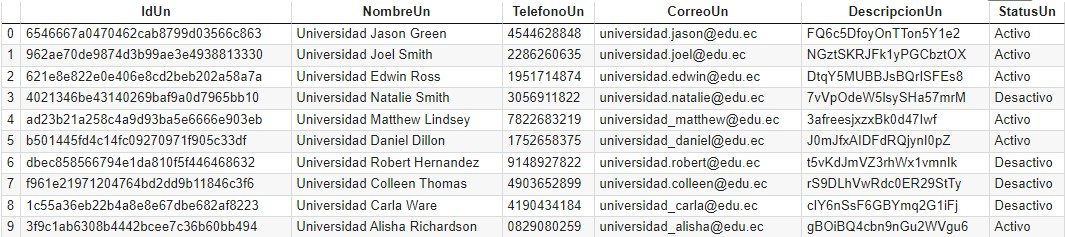
\includegraphics[width=1\columnwidth]{TablaUniversidad.jpg}
        \caption{\label{fig1}Entidad Universidad.
        }
\end{figure}

La figura~\ref{fig2} es la representación de la entidad Permisos donde se puede observar los diez primeros datos de los 5 mil generádos. Además, en este se puede observar como cada identificador tiene un permiso asignado ya sea leer, editar, subir o eliminar. Si bien estos no son todos los datos, podremos encontrar el csv en un repositorio de github público donde podremos encontrar todos los 5 mil datos sinéticos generados~\cite{permiso,permisocsv}.

\begin{figure}[H] 
        \centering 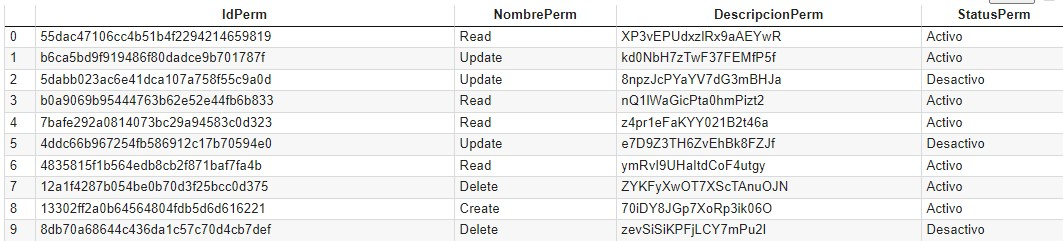
\includegraphics[width=1\columnwidth]{TablaPermisos.jpg}
        \caption{\label{fig2}Entidad Permisos.
        }
\end{figure}

La figura~\ref{fig3} es la representación de la entidad Puntaje, cada uno con sus datos relacionados a los atributos que contiene la entidad. Por ejemplo, podemos observar como se generó notas en los diez primeros datos en el rango que se especificó de 400 a 1000 puntos. Si bien estos no son todos los datos, podremos encontrar el csv en un repositorio de github público donde podremos encontrar todos los 5 mil datos sinéticos generados~\cite{puntaje,puntajecsv}.

\begin{figure}[H] 
        \centering 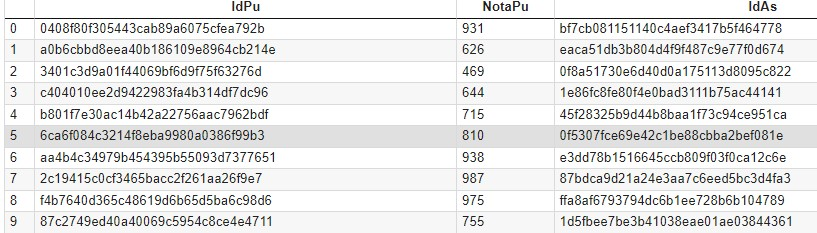
\includegraphics[width=1\columnwidth]{TablaPuntaje.jpg}
        \caption{\label{fig3}Entidad Puntaje.
        }
\end{figure}

La figura~\ref{fig4} es la representación de la entidad Usuarios, donde se observa sus cuatro atributos mencionados en la sección anterior. La entidad usuarios por ejemplo, serán los encargados de llevar una administración en la base de datos relacional. Por ejemplo, en el caso del tipo de usuario tenemos tres tipos, 3 para Administrador/a, 2 para secretario/a y 1 para Call Center. Si bien estos no son todos los datos, podremos encontrar el csv en un repositorio de github público donde podremos encontrar todos los 5 mil datos sinéticos generados~\cite{usuario,usuariocsv}.

\begin{figure}[H] 
        \centering 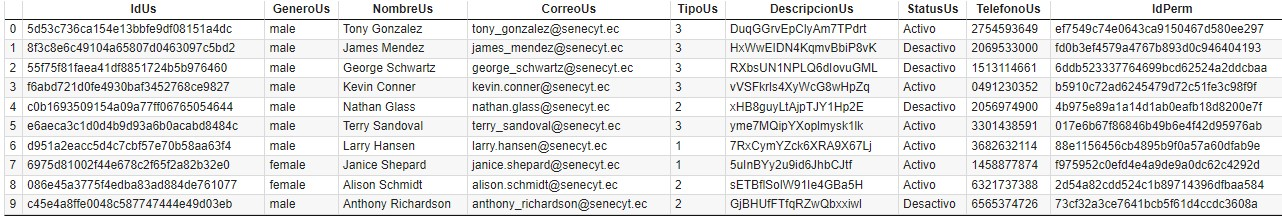
\includegraphics[width=1\columnwidth]{TablaUsuarios.jpg}
        \caption{\label{fig4}Entidad Usuarios.
        }
\end{figure}

\section{Discusión}
En el presente laboratorio se encontró las distintas entidades a tomar en cuenta en el proyecto a realizar sobre los puntajes referenciales de la Senecyt. Además, se tomo en cuenta cada uno de sus atributos en cada entidad. Se hallo en el laboratorio como obtener los datos sintéticos necesarios y como obtenerlos mediante la programación en el lenguaje de Python, junto con la herramienta Colab, la cual aprendimos qué esta nos brinda las librerías necesarias para la exportación e imputación de datos sintéticos. Se consideró, la carga necesaria a cada entidad para su análisis en un futuro, que nos ayudará a construir la base de datos relacional. Uno de los grandes problemas que se encontró, es que Python maneja mucho la orientación de objetos, por lo cual, se consideró aprender mediante una investigación un poco más sobre este lenguaje para poder generar bien los scripts que se necesitaron en este laboratorio. 

El lenguaje de programación de Python, es una lenguaje muy didáctico al momento de genérar en este caso datos sintéticos. Python nos proporciona una serie de librerías donde nos facilitan el desarrollo de las aplicaciones o sistemas. Colab es una herramienta donde sirve como emulador del lenguaje de programación que a pesar de sus limitaciones, tenemos un amplio porcentaje de almacenamiento, que a pesar de todo el código que se generó no proporcionó grandes problemas a lo largo de este desarrollo.

En cada uno de las 4 entidades que son Univesidad, Puntaje, Permiso y Usuario, se tomo muy en cuenta que cada uno debe tener características únicas, en el cual el usuario pueda verificar qué no todas tienen la misma funcionalidad. si bien, un atributo puede ser parecido entre entidades, se debe considerar en los datos la forma de caracterizar mediante un análisis las características a tomar en cuenta. Así, nuestra tabla de resultados tendran datos sintéticos limpios, para un mejor análisis en la problemática general. 

Mediante la apreciación de tablas de datos, nos podémos fijar los valores que van tomando cada uno de las filas en cada atributo mencionado anteriormente. Los datos deben ser limpios en una tabla, ya que, esta tabla es donde se evidenciará el análisis que se ha hecho durante todo el laboratorio. Sin embargo, hay que tomar en consideración, que no todos los datos pueden ser totalmente limpios por lo cual eso conlleva a un futuro a analizar los datos sintéticos para así poder obtener totalmente una tabla bien desarrollada.

\section{Conclusión}
En conclusión, Python es un lenguaje fácil de usar y de aprender, que mediante su libertar al acceso de las tantas librerías que contiene se puede desarrollar el objetivo principal de una base de datos relacional, embarcándola al proyecto. Sin embargo, hay que tomar en cuenta que el desarrollo de unos datos sintéticos no solo basta con saber programar, si no, también hay que tomar en cuenta mucho el análisis que se necesita para abarcar todos los requerimientos del laboratorio y del proyecto. En resumen, los datos relacionales son importantes en el análisis y desarrollo del proyecto, ya que, estos serán los que nos brinden la información necesaria para culminar con los objetivos planteados en el proyecto. 

\nocite{*}
\bibliographystyle{plain}
\bibliography{paper}
\end{document}  
